% CVSId: $Id: lctes03-talk.tex,v 1.17 2003-06-02 20:10:25 cananian Exp $
%%%%%%%%%%%%%%%%%%%%%%%%%%%%%%%%%%%%%%%%%%%%%%%%%%%%%%%%%%%%%%%%%%%%%%%%%
% TO DO:
%%%%%%%%%%%%%%%%%%%%%%%%%%%%%%%%%%%%%%%%%%%%%%%%%%%%%%%%%%%%%%%%%%%%%%%%%
%  X a slide to explain loops/our choice opposed to interval analysis KILL
%  - Trim ``Intraprocedural analysis'': jump to bitwidth, focus on
%    information gained, not process by which it is obtained
%    kill example, define latice algebraically
%  - Explain (spend more time on) how the *inter* procedural analysis
%    works/how fields are treated.  A graphic here?
%  - Prettify the ``field packing'' slide.
%  - Use solid colors on results slides.
%  - Helvetica font on title slide
%  - ``We'd love to do embedded benchmarks''
%%%%%%%%%%%%%%%%%%%%%%%%%%%%%%%%%%%%%%%%%%%%%%%%%%%%%%%%%%%%%%%%%%%%%%%%%
\documentclass[%
pdf,
colorBG,
slideColor,
%nocolorBG,
%slideBW,
%%%%%%%%%%%%%%%%%%%%%
nototal,
%distiller,
%%%%%%%%%%%%%%%%%%%%%
%draft,
oqe
%frames
%azure
%contemporain
%nuancegris
%troispoints
%lignesbleues
%darkblue
%alienglow
%autumn
]{prosper}
\usepackage{amsmath}
\usepackage{comdef}\newcommand{\figscale}{1.0}
\usepackage{pst-node}
\usepackage{verbatim}
%\hypersetup{pdfpagemode=FullScreen}

\slideCaption{Ananian/LCTES'03}
\title{Size Optimizations for Java Programs}
\author{\large\href{http://cscott.net}{C.~Scott~Ananian} and \href{http://www.cag.lcs.mit.edu/~rinard}{Martin~Rinard}}
\email{\{\href{mailto:cananian@lcs.mit.edu}{cananian},\href{mailto:rinard@lcs.mit.edu}{rinard}\}@lcs.mit.edu}
\institution{%
Laboratory for Computer Science\\
Massachusetts Institute of Technology
\\
\vspace{.5cm}
LCTES'03, June 2003
}

%\DefaultTransition{Wipe}
\renewcommand{\yellow}{\colC}
\ifDVItoPS\renewcommand{\white}{\black}\fi
\newcommand{\betweenSlide}[3]{\fromSlide{#1}{\untilSlide{#2}{#3}}}
\newenvironment{mysamplecode}{\small\bfseries\begin{samplecode}}{\end{samplecode}}
\newcommand{\func}[1]{\ensuremath{\text{\sffamily\bfseries #1}}}
% Meet symbol
\newcommand{\meet}{\ensuremath{\sqcap}}
% lattice inequalities
\newcommand{\latlt}{\ensuremath{\sqsubset}}
\newcommand{\latleq}{\ensuremath{\sqsubseteq}}
% absolute value, with proper brackets
\providecommand{\abs}[1]{\lvert#1\rvert}

%%%%% define new 'talknotes' environment that only shows up in PS mode.
\ifDVItoPS
\newenvironment{talknotes}{\begin{slide}{Notes}\tiny}{\end{slide}}
\else
% this redefinition of talknote to be == comment is from an example in
% the verbatim package (where the comment environment comes from).
\let\talknotes=\comment
\let\endtalknotes=\endcomment
\fi

\begin{document}
\maketitle

\begin{talknotes}
Nothing should be said on the title slide.
\end{talknotes}

%---------------------------------------------------------------------- SLIDE -
\begin{slide}{Our Goal}
\begin{center}
Reduce the memory consumption of object-oriented programs

\vspace{0.5cm}
\fontTitle{By}
\vspace{0.5cm}

Using program analysis to identify opportunities to reduce the space
required to store objects,

\vspace{0.5cm}
\fontTitle{Then}
\vspace{0.5cm}

Applying transformations to reduce the memory consumption of the program.
\end{center}
\end{slide}

\begin{talknotes}
This talk is about size optimizations for Java programs.  Our goal is
to reduce the amount of memory used by object-oriented programs (in
this case, Java) by using static whole-program analyses to identify
opportunities and applying transformations to effect the reduction.
\end{talknotes}

%---------------------------------------------------------------------- SLIDE -
\overlays{8}{
\begin{slide}{Why space optimizations?}
\begin{itemize}
 \FromSlide{2}
 \item Embedded applications:
 \FromSlide{3}
 \begin{itemize}
  \item Better use of {\yellow existing fixed memory resources}.
  \FromSlide{4}
  \item \bp{\yellow Reduce memory costs} of new devices.
 \end{itemize}
 \FromSlide{5}
 \item Performace:
 \FromSlide{6}
 \begin{itemize}
  \item ``{\yellow Memory wall}'' getting higher.
  \FromSlide{7}
  \item Space optimizations increase the {\yellow effective cache size},
  improving performance.
  \FromSlide{8}
  \item Added {\yellow ALU ops} getting comparatively {\yellow cheaper}.
 \end{itemize}
\end{itemize}
\end{slide}
}

\begin{talknotes}
XXX: write me.
\end{talknotes}

%---------------------------------------------------------------------- SLIDE -
\begin{slide}{Structure of a Java Object}
\begin{itemize}
\item Typical of many O-O languages.
\end{itemize}
\begin{center}
\includegraphics[scale=0.5]{Figures/Kontour/structure-bbox.eps}
\end{center}
\end{slide}

\begin{talknotes}
Here's our starting point.  This is how most Java implementations lay
out objects.  I want you to notice that there are three kinds of space
in this layout, helpfully delineated with red lines.  The first
section of the object usually consists of information required by
the runtime implementation but not directly specified by the
programmer.  This includes a claz pointer, which points to an
external structure of information about the object's type, and
some information to support the hashcode and locking semantics of
Java.  % Every object has a hashcode and can be locked upon, etc, etc.
The second section of the object contains the fields declared by
the programmer.  If this were a car object, these fields might
indicate the color and model of the car.  The last section
consists of padding which the runtime implementation will
add to bring the various parts of the object to certain alignment
boundaries.
\end{talknotes}

%---------------------------------------------------------------------- SLIDE -
\newrgbcolor{fieldcomp}{0 1 0}
\newrgbcolor{fieldelim}{0 1 1}
\newrgbcolor{headeropt}{1 0 1}

\overlays{4}{%
\begin{slide}{How to compress objects} %

Three broad techniques:
%
\parbox[b]{2.5in}{%
\fromSlide{2}{
\begin{itemize}%
\fieldcomp\renewcommand{\green}{\fieldcomp}% new bullet color
\item Field compression
\fromSlide{3}{
\fieldelim\renewcommand{\green}{\fieldelim}% new bullet color
\item Mostly-constant field elimination
\fromSlide{4}{
\headeropt\renewcommand{\green}{\headeropt}% new bullet color
\item Header optimizations
}}
\renewcommand{\green}{\yellow} % restore yellow bullet color
\end{itemize}
}}%
\parbox[b]{1.75in}{%
\onlySlide*{1}{\hspace*{0.106in}\hspace*{0.261in}\includegraphics[scale=0.4]{Figures/Kontour/how-none-bbox.eps}}%
\onlySlide*{2}{\hspace*{0.106in}\hspace*{0.261in}\includegraphics[scale=0.4]{Figures/Kontour/how-fieldcomp-bbox.eps}}%
\onlySlide*{3}{\hspace*{0.106in}\includegraphics[scale=0.4]{Figures/Kontour/how-fieldelim-bbox.eps}}%
\onlySlide*{4}{\includegraphics[scale=0.4]{Figures/Kontour/how-header-bbox.eps}}%
}%

\end{slide}
}

\begin{talknotes}
There are three broad techniques we are going to use to effect our
size reductions: @ field compression, which reduces the size of the
programmer-declared fields and the padding between fields,
@ mostly-constant field
elimination, to completely eliminate memory used to store common values,
and @ header optimizations, which leverage more-efficient
representations for the data needed by the runtime.  We will look at each
of these in order, starting with\ldots
\end{talknotes}

%---------------------------------------------------------------------- SLIDE -
\overlays{1}{% work around spacing bug in \overlays
\begin{slide}{How to compress objects} % just the first one

Three broad techniques:
%
\parbox[b]{2.5in}{%
\begin{itemize}%
\fieldcomp\renewcommand{\green}{\fieldcomp}% new bullet color
\item Field compression
\lightgray\renewcommand{\green}{\lightgray}% new bullet color
\item Mostly-constant field elimination
\lightgray\renewcommand{\green}{\lightgray}% new bullet color
\item Header optimizations
\renewcommand{\green}{\yellow} % restore yellow bullet color
\end{itemize}
}%
\parbox[b]{1.75in}{%
\hspace*{0.106in}\hspace*{0.261in}\includegraphics[scale=0.4]{Figures/Kontour/how-fieldcomp-bbox.eps}%
}%
\end{slide}
}

\begin{talknotes}
\ldots field compression.
\end{talknotes}

%---------------------------------------------------------------------- SLIDE -
\newsavebox{\blbox}
\overlays{6}{
\begin{slide}{Field Compression}
Reduce the space taken up by an object's fields.
\begin{itemize}
\fromSlide{2}{
\item \bp{\yellow Sparse Predicated Typed Constant analysis} to
  discover unread/unused/constant fields.
\fromSlide{4}{
\item \bp{\yellow Bitwidth analysis} to discover tight upper bounds on
  field size.
\fromSlide{6}{
\item \bp{\yellow Field packing} into bytes or bits.
}}}
\end{itemize}

\framebox{\parbox{2in}{%
\begin{mysamplecode}%
class Car \{\\
\>int color;\\
\>\ldots\\
\}\\
\end{mysamplecode}%
}%
\parbox{3in}{%
\fromSlide{3}{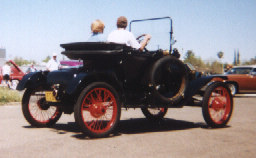
\includegraphics[height=.8in]{Figures/Images/model-t-black.eps}}
\fromSlide{5}{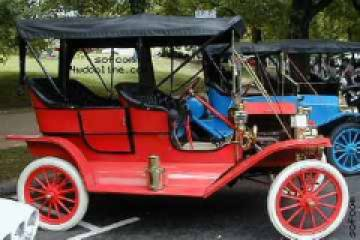
\includegraphics[height=.8in]{Figures/Images/model-t-redblue.eps}}\\
\tt\bfseries%
% the \sbox below would let us put black text on a white back if we
% felt like it.
~\fromSlide{3}{\sbox{\blbox}{BLACK=0}\white\usebox{\blbox}}%
~\fromSlide{5}{{\red RED=1}~{\blue BLUE=2}}
}%
}

\end{slide}
}

\begin{talknotes}
Field compression targets the space directly allocated by the
programmer.  In the sample class at the bottom of the slide, we
define an object representing cars.  Its first field is a color,
and it is declared an integer which allows the enumeration of up
to $2^{32}$ different colors of cars.

@ The first analysis we do is a standard sparse conditional constant
propagation pass over the whole program to identify unused, unread,
or constant fields.  @ Suppose we're building Ford Model-T's.
Since they only come in black, this field will be constant and
can be removed.

@ A novel contribution is the next step, bitwidth analysis, which discovers
tighter upper bounds on field sizes.  @  Actually, Model-T's were
produced in several different colors before Ford started
mass-production.  Our bitwidth analysis could determine that
we really only need two bits to store colors, since our program
only ever stores three different colors in a Car object.

@ After we perform the analysis, we use the results to
reduce the space used by the fields.  We'll talk about this later.

~%
\end{talknotes}

%---------------------------------------------------------------------- SLIDE -
\part{How are these analyses performed?}
\begin{talknotes}
So how do we actually obtain the information we need to do field
compression?

~%
\end{talknotes}

%---------------------------------------------------------------------- SLIDE -
\begin{slide}{Bitwidth analysis domains}
Domains:
\begin{itemize}
\item $\mathcal{C}:\mathbb{Z}$, integer constants
\begin{itemize}\yellow
\item $c\in\mathcal{C}$
\end{itemize}
\item $\mathcal{T}:\mathbb{N}_0\times\mathbb{N}_0$, bitwidth specifications
 %% FIXME: should be on same line as previous.
 ($\mathbb{N}_0=\left\{0,1,2,\ldots\right\}$)
\begin{itemize}\yellow
\item $\tuple{m,p}\in\mathcal{T}$
\end{itemize}
\item $\mathcal{L}:\left(\mathcal{C+T}\right)_\bot$, abstract value lattice
\end{itemize}
Concretization: $\mathcal{L}\to 2^\mathcal{Z}$
\begin{eqnarray*}
\mathbb{C}\left[c\right] &=& \left\{ c \right\} \\
\mathbb{C}\left[\tuple{m,p}\right] &=&
   \left\{ -n | n\in\mathbb{N}_0 \,\wedge\, \ln n < m\right\} \cup
   \left\{0\right\} \cup\\
&& \left\{  n | n\in\mathbb{N}_0 \,\wedge\, \ln n < p\right\}\\
\end{eqnarray*}
\end{slide}

\begin{talknotes}
Let's first establish some domains we need for the bitwidth analysis.
Our abstract lattice domain $\mathcal{L}$ will include integer constants,
represented by the domain $\mathcal{C}$ as well a domain $\mathcal{T}$
of tuples of non-negative integers.  The $\mathcal{T}$ domain
represents bitwidth constraints, split into negative and positive
parts.  The first member of the tuple, $m$, will represent the
bitwidth of any possible negative values, and the second member, $p$
will represent the bitwidth of positive values.

Our lattice of abstract values for the bitwidth analysis will range
over the raised sum of $\mathcal{C}$ and $\mathcal{T}$.

~%
\end{talknotes}

%---------------------------------------------------------------------- SLIDE -
\overlays{5}{
\begin{slide}{Ordering relationships in $\mathcal{L}$}%
{\onlySlide*{1}{\yellow}%
 For all $c\in\mathcal{C}$, $\tuple{m,p}\in\mathcal{T}$:}%
\begin{eqnarray*}%
\bot\latleq c &\text{ and }& \bot\latleq\tuple{m,p}\\
\tuple{m_1,p_1}\latleq\tuple{m_2,p_2}&\text{ iff }&m_1\leq m_2 \wedge p_1\leq p_2\\
c\latleq\tuple{m,p}&\text{ iff }&\func{bw}(c)\latleq\tuple{{\onlySlide*{5}{\yellow}m},{\onlySlide*{4}{\yellow}p}}
\end{eqnarray*}%
\FromSlide{2}%
\begin{flushleft}\onlySlide*{2}{\yellow}where:\end{flushleft}
\begin{displaymath}%
\func{bw}(c):\mathcal{C}\to\mathcal{T}=\begin{cases}
\tuple{0,0} & c=0 \\
\tuple{0,{\onlySlide*{4}{\yellow}1+\left\lfloor\ln\abs{c}\right\rfloor}} & c>0 \\
\tuple{{\onlySlide*{5}{\yellow}1+\left\lfloor\ln\abs{c}\right\rfloor},0} & c<0 \\
\end{cases}%
\end{displaymath}%
\FromSlide{3}%
\begin{displaymath}%
\begin{array}{ccc}
\text{\tt 0\ldots 0}\overbrace{\text{\tt 1X\ldots XXX}}^{1+\left\lfloor\ln\left|c\right|\right\rfloor\fromSlide{4}{\onlySlide*{4}{\yellow}=p}}
&\quad&
\text{\tt 1\ldots 1}\overbrace{\text{\tt 0X\ldots XXXX}}^{1+\left\lfloor\ln\left(\left|c\right|-1\right)\right\rfloor\fromSlide{5}{\onlySlide*{5}{\yellow}\leq m}}
\\
\text{\small Positive} && \text{\small Negative}
\end{array}
\end{displaymath}
\end{slide}
}

\begin{talknotes}
Now we will define the ordering relationship on $\mathcal{L}$.  The
$\bot$ value will represent ``no information'' and is less than all
members of $\mathcal{C}$ and $\mathcal{T}$ in the lattice.  Members of
$\mathcal{T}$ are compared component-wise; a bitwidth is lesser only
if both its components are lesser.  Finally, a constant $c$ is lesser
only if the function $\func{bw}$ of $c$ is less-than-or-equal,
@ where $\func{bw}(c)$ computes the number of bits needed to
represent the signed constant $c$.  @ For values in twos complement
notation, @ the $p$ component of the result represents the location of
the first one in the number, and the @ $m$ component constrains the
location of the first zero.
\end{talknotes}

%---------------------------------------------------------------------- SLIDE -
\overlays{6}{
\begin{slide}{Some abstract evaluation rules}
\begin{eqnarray*}
\onlySlide*{2}{\yellow}%
\text{\tt -}\tuple{m,p}
 &\onlySlide*{2}{\yellow}=&\onlySlide*{2}{\yellow}%
 \tuple{p,m}
 \\
\onlySlide*{3}{\yellow}%
\tuple{m_l,p_l} \text{\tt+} \tuple{m_r,p_r}
 &\onlySlide*{3}{\yellow}=&\onlySlide*{3}{\yellow}%
 \tuple{1+\max(m_l,m_r),1+\max(p_l,p_r)}
 \\
\onlySlide*{4}{\yellow}%
\tuple{m_l,p_l} \text{\tt *} \tuple{m_r,p_r}
 &\onlySlide*{4}{\yellow}=&\onlySlide*{4}{\yellow}%
\tuple{\begin{array}{l}\max(m_l+p_r,p_l+m_r),\\
                       \max(m_l+m_r,p_l+p_r)\end{array}}
 \\
\onlySlide*{5}{\yellow}%
\tuple{0,p_l} \text{\tt\&} \tuple{0,p_r}
 &\onlySlide*{5}{\yellow}=&\onlySlide*{5}{\yellow}%
 \tuple{0,\min(p_l,p_r)}
 \\
\onlySlide*{6}{\yellow}
\tuple{m_l,p_l}\text{\tt\&} \tuple{m_r,p_r}
 &\onlySlide*{6}{\yellow}=&\onlySlide*{6}{\yellow}%
 \tuple{\max(m_l,m_r),\max(p_l,p_r)}
 \\
\end{eqnarray*}
\end{slide}
}

\begin{talknotes}
Here are some of the abstract evaluation rules we use for
unary and binary operations over
our bitwidth value domain.

@ The first entry simply says that negation
exchanges the positive and negative bitwidths.
The symmetric definition for our negative and positive
bitwidths which you saw in the previous slide, where we 
tracking the bitwidth of the \textit{absolute value} of the number,
we chosen so that we don't lose information in this rule.

@ The second entry gives
the rules for addition: we have to add one to the width to allow for
carry out.

@ The rule for multiplication should remind you that we're
operating in the log-domain.  

@ The underlying numeric representation
shows through in our rules for logical-AND; this first rule is a
special-case for ANDing two positive values.  The result will always
be positive, and leading zeros in the smaller number will always force
leading zeros in the result.

@ If either value can be negative, the result must be more
pessimistic, because every negative range includes the ``all-ones''
value $-1$.  We don't have time to justify this rule in detail, but it
is in the paper and you can check it at your leisure.

~%force rejust.
\end{talknotes}

%---------------------------------------------------------------------- SLIDE -
\begin{slide}{Intraprocedural bitwidth analysis}
\begin{itemize}
\item Given domains:
\begin{itemize}
\item $\mathcal{E}$, CFG edges
\item $\mathcal{V}$, (SSI form) variables
\end{itemize}
\item The intraprocedural analysis discovers:
\begin{itemize}
\item a set $\func{e}:2^\mathcal{E}$ of executable edges
\item a map $\func{val}:\mathcal{V}\to\mathcal{L}$ giving abstract
  values valid for all possible executions
\end{itemize}
\end{itemize}
\end{slide}

\begin{talknotes}
The result of our intraprocedural bitwidth analysis gives a set $e$ of
executable edges, and a mapping from all variables to a lattice
element constraining their values in all possible program executions.
\end{talknotes}

%---------------------------------------------------------------------- SLIDE -
\overlays{2}{
\begin{slide}{SSI form}
Allows us to discover facts about \texttt{i} at points \textit{A} and
\textit{B}:
\begin{mysamplecode}
i\onlySlide{2}{{\yellow$_0$}}= \ldots;\\
\ldots\\
i\onlySlide{2}{{\yellow$_1$}}= \ldots;\\
while (0<i\onlySlide{2}{{\yellow$_1$}} \&\& i\onlySlide{2}{{\yellow$_1$}}<50) \{\\
\>\ldots=i\onlySlide{2}{{\yellow$_2$}}; \it// A\\
\}\\
\ldots=i\onlySlide{2}{{\yellow$_3$}}; \it// B\\
\end{mysamplecode}
\FromSlide{2}
\vspace{.75cm}
\begin{center}\yellow
$\func{val}(\text{\tt i}_2)\latleq\langle 0,\underbrace{6}_{1+\lfloor\ln 50\rfloor}\rangle$
\end{center}
\end{slide}
}

\begin{talknotes}
The SSI form is a variant of SSA form which @ allows us to distinguish
the values produced in the two different assignments to {\tt i} at the
start of this example, as well as distinguish the possible values of
{\tt i} at point {\it A} ($\tuple{0,6}$) and at point {\it B}.
\end{talknotes}

%---------------------------------------------------------------------- SLIDE -
\begin{slide}{Interprocedural analysis}
We use a {\yellow field-based} interprocedural analysis.
\begin{itemize}
\item Given domains:
\begin{itemize}
\item $\mathcal{E}$, CFG edges
\item $\mathcal{V}$, (SSI form) variables
\item $\mathcal{F}$, declared fields in the program
\end{itemize}
\item The interprocedural analysis discovers:
\begin{itemize}
\item a set $\func{e}:2^\mathcal{E}$ of executable edges
\item a map $\func{val}:(\mathcal{V}+\mathcal{F})\to\mathcal{L}$
 giving abstract values valid for all possible executions
\item a set $\func{Read}:2^\mathcal{F}$ of readable fields
\end{itemize}
\end{itemize}
\end{slide}
% XXX add domain M, declared methods, and change type of val to
% (F+(VxM*))->L ?
\begin{talknotes}
We extend our intraprocedural analysis interprocedurally using a
field-based scheme.  The domain $\mathcal{F}$ represents the declared
fields of the program, and our value map $\func{val}$ now maps not
only variables but also fields to lattice values.  We also collect a
set $\func{Read}$ of fields read by executable statements in the
program to allow us to eliminate unread fields.
\end{talknotes}

%---------------------------------------------------------------------- SLIDE -
\begin{slide}{All cars are black}
\vspace{1cm}
\begin{samplecode}
void paint(int color) \{\\
\>if (this.model == FORD)\\
\>\>color = BLACK;\\
\>this.color = color;\\
\}\\
\end{samplecode}
\end{slide}

\begin{talknotes}
Returning to our car example, we can see how our initial Sparse
Predicated Typed Constant analysis could determine that, if all cars'
model is FORD, then all car's color will be BLACK.  Having determined
this, we can simply substitute BLACK for the color wherever it appears
and remove the field.  However, if there are non-FORD cars, we can
still use our bitwidth analysis to determine a bound on how many
bits we need to represent the various car colors that we see assigned
to the color field.
\end{talknotes}

%---------------------------------------------------------------------- SLIDE -
\begin{slide}{{\small Using the analysis:}\\
              Field compression using bitwidths}

\begin{center}
\vspace{1cm}
\includegraphics[scale=0.5]{Figures/Kontour/bwfieldcomp-bbox.eps}
\end{center}
\end{slide}

\begin{talknotes}
Now we're going to show how the analysis results are used to transform
the program.

Once we've used our analysis to determine accurate widths for fields,
we would like to shrink the objects' allocations to use only the space
actually needed for each field.  So if we have less than 256 colors,
we can use a single byte in the object structure to represent color.
\end{talknotes}

%---------------------------------------------------------------------- SLIDE -
% \begin{slide}{Field packing}
% \centering\small
% \begin{tabular}{|l|}
% \hline
% Standard packing word-aligns the object and aligns each field to the
% width of its type (4-byte data is 4-byte aligned):\\
% 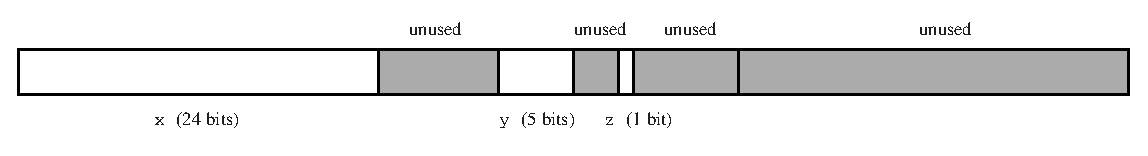
\includegraphics[scale=0.7]{Figures/standardAlignment.eps}\\
% ``Byte'' alignment byte-aligns the object and all fields:
% \hfill\raisebox{-1ex}[0pt][0pt]{\parbox[t]{3in}{
% \begin{samplecode}
% class A \{\\
% \>int x;  /* actual width 24 bits */\\
% \>byte y; /* actual width 5 bits */\\
% \>boolean z; /* actual width 1 bit */\\
% \}\\
% \end{samplecode}
% }}\\
% 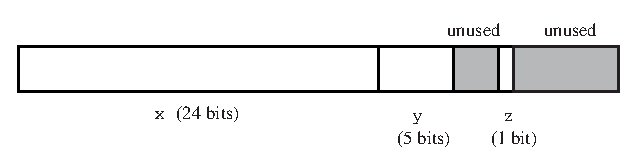
\includegraphics[scale=0.7]{Figures/byteAlignment.eps}\\
% ``Bit'' alignment requires no alignment of objects or fields:\\
% 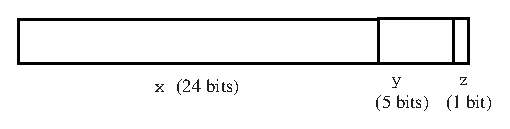
\includegraphics[scale=0.7]{Figures/bitAlignment.eps}\\
% \hline
% \end{tabular}

% Object header omitted.
% \end{slide}

%---------------------------------------------------------------------- SLIDE -
\begin{slide}{Field packing}
% converted with pngtopnm Figures/alignment.png | pnmtops -equalpixels -noturn > Figures/alignment.eps
\begin{center}
\vspace{0.75cm}
%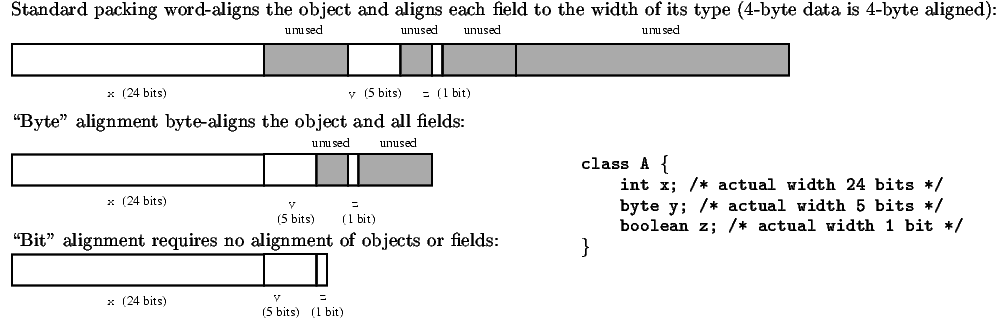
\includegraphics[scale=1.3]{Figures/alignment.eps}
\includegraphics[scale=0.35]{Figures/alignment2.eps}
%\includegraphics[scale=0.35]{Figures/alignment3.eps}

\small Object header omitted.
\end{center}
\end{slide}

\begin{talknotes}
The actual situtation is a little more complicated.  There is padding
within and at the end of the object, required for various reasons.
The heap allocator may prefer to have the chunks it returns aligned
on certain boundaries, and the machine architecture may prefer to
access, for example, word data aligned at word boundaries.  At
some runtime cost, we can overcome these limitations.  At the top, is
the standard ``Java'' object packing.  All fields are aligned to their
natural size, so that, word-sized fields will always begin at word
boundaries.  In this work we implemented a ``byte'' alignment
strategy, where all fields are placed at the nearest \emph{byte}
boundaries, irrespective of their preferred alignment.  One can also
imagine a ``bit'' alignment strategy where each field uses
\emph{exactly} the number of bits it requires.  At runtime we must
then perform bit-masking and -extraction operations to access the
fields.  We found very little additional space-savings potential from
going to bit alignment, which is why the numbers we will present use
``byte'' alignment.

~%
\end{talknotes}

%---------------------------------------------------------------------- SLIDE -
\begin{slide}{How to compress objects} % just the second one

Three broad techniques:

\parbox[b]{2.5in}{%
\begin{itemize}%
\lightgray\renewcommand{\green}{\lightgray}% new bullet color
\item Field compression
\fieldelim\renewcommand{\green}{\fieldelim}% new bullet color
\item Mostly-constant field elimination
\lightgray\renewcommand{\green}{\lightgray}% new bullet color
\item Header optimizations
\renewcommand{\green}{\yellow} % restore yellow bullet color
\end{itemize}
}%
\parbox[b]{1.75in}{%
\hspace*{0.106in}\includegraphics[scale=0.4]{Figures/Kontour/how-fieldelim-bbox.eps}%
}%
\end{slide}

\begin{talknotes}
Let's return to our outline.  So far we have talked about field
compression; using bitwidth analysis to reduce the static size of
fields allocated in objects, and using field packing to reduce the
amount of object padding.  Now we will talk about ``Mostly-constant
field elimination,'' our second space-reduction technique.
\end{talknotes}

%---------------------------------------------------------------------- SLIDE -
\overlays{6}{
\begin{slide}{Mostly-constant field elimination}
\begin{itemize}
 \item It's easy to remove {\yellow constant} fields.
 \fromSlide{2}{
 \item Key idea: remove \textit{\yellow mostly} constant fields.
 \fromSlide{3}{
 \begin{itemize}
  \item \bp{\yellow Identify} fields which have a certain value ``most of
        the time.''
  \fromSlide{4}{
  \begin{itemize}
   \item \small Static analysis/profiling.
  \end{itemize}
  \fromSlide{5}{
  \item \bp{\yellow Transform} objects to remove fields w/ the common
        value.
  \fromSlide{6}{
  \begin{itemize}
   \item \small Static specialization/externalization.
  \end{itemize}
  }}}
 \end{itemize}
 }}
\end{itemize}
\end{slide}
}

\begin{talknotes}
It's easy to remove constant fields; we just replace the field
reference with the appropriate constant.  @ But our key idea here is
that it is also possible to replace \emph{mostly}-constant fields.
@ We identify fields which have a certain value ``most of the time''
using @ static analysis and profiling.  @ We can then transform the
objects to remove fields with the common value, so that we only
spend space on fields with unusual values.  @ Our techniques for doing
this are called static specialization and externalization.
The types of ``mostly-constant'' fields that can be removed are
slightly different with the two techniques; we will look at static
specialization first.
\end{talknotes}

%---------------------------------------------------------------------- SLIDE -
\begin{slide}{Specialization example:\\\small java.lang.String}
\fontsize{9}{9}%
\bfseries\begin{samplecode}%
public final class String \{\\
\>private final char value[];\\
\>private final int offset;\\
\>private final int count;\\
\>\ldots\\
\>public char charAt(int i) \{\\
\>\>return value[offset+1];\\
\>\}\\
\>public String substring(int start) \{\\
\>\>int noff = offset + start;\\
\>\>int ncnt = count - start;\\
\>\>return new String(value, noff, ncnt);\\
\>\}\\
\}\\
\end{samplecode}
\end{slide}

\begin{talknotes}
We're going to jump right in with an example.  This is {\tt
  java.lang.String} from the Java standard class library.  It has
three fields: a character array and an integer length and offset.
This representation was chosen to allow you to perform the substring
operation in constant time; you don't have to copy the string, you
just create a new string with a different offset and length and
share the same character array.

The interesting thing about {\tt java.lang.String} is that the {\tt
  offset} field is almost \emph{always} zero.  Only strings created
with the {\tt substring()} method have non-zero offset fields. 
And the offset field is never changed after the object is created.
These are the key properties needed to enable static specialization.
\end{talknotes}

%---------------------------------------------------------------------- SLIDE -
\begin{slide}{Key properties}
To use static specialization we need:
\begin{itemize}
 \item A field with a frequently-occuring value.
  \begin{itemize}\small
   \item {\tt\bfseries String.offset} is almost always zero.
  \end{itemize}
 \item The value of the field must never be modified after the object
       is created.
\end{itemize}
\end{slide}

\begin{talknotes}
In order to apply our technique, we need to find a ``mostly-constant''
field, which in our example is {\tt String.offset}, with the value
``mostly zero'', and, importantly, the value of that field cannot be
modified after the object is created.
\end{talknotes}

%---------------------------------------------------------------------- SLIDE -
\overlays{4}{
\begin{slide}{Transforming the class}
We will split String into two classes:
\begin{itemize}
\item {\tt\bfseries\yellow SmallString} without the field.
\item {\tt\bfseries\yellow BigString} with the field.
\end{itemize}

We will use {\tt\bfseries SmallString} for all instances where
the offset field is zero (our ``mostly-constant'' value).

\vspace{1cm}
\FromSlide{2}
{\yellow Problems:}
\FromSlide{3}
\begin{itemize}
 \item The code could directly access the to-be-removed field.
 \fromSlide{4}{%
 \item Allocation sites directly instantiate the old class.
 }
\end{itemize}
\end{slide}
}

\begin{talknotes}
So, how are we going to save memory in {\tt java.lang.String}?
We're going to split the class in two: there will be a {\tt
  SmallString} class without the offset field, and a {\tt BigString}
class that does have it.

@ A couple of problems that come up:
\begin{itemize}
\item @ What happens to places in {\tt SmallString} where the removed
offset field is referenced?
\item @ And when we see an allocation of {\tt String}, do we change it
to {\tt SmallString} or {\tt BigString}?
\end{itemize}
\end{talknotes}

%---------------------------------------------------------------------- SLIDE -
\overlays{3}{
\begin{slide}{Specialization example:\\\small java.lang.String}
\fontsize{9}{9}%
\newcommand{\myOffset}{\onlySlide*{1}{offset}\onlySlide*{2}{offset}%
%{\makebox[0pt][l]{offset}}
\onlySlide*{3}{{\yellow getOffset()}}}%
\bfseries\begin{samplecode}%
public final class \onlySlide*{1}{String}\fromSlide*{2}{\yellow SmallString} \{\\
\>private final char value[];\\
\pnode{offl}%
\>private final int offset;%
\pnode{offr}\\
\>private final int count;\\
\onlySlide{3}{\>\yellow protected int getOffset() \{ return 0; \}}\\
\>\ldots\\
\>public char charAt(int i) \{\\
\>\>return value[\myOffset{}+1];\\
\>\}\\
\>public String substring(int start) \{\\
\>\>int noff = \myOffset{} + start;\\
\>\>int ncnt = count - start;\\
\>\>return new String(value, noff, ncnt);\\
\>\}\\
\}\\
\end{samplecode}
\fromSlide*{2}{\ncline[linecolor=red,linewidth=2pt]{offl}{offr}}%
\end{slide}
}

\begin{talknotes}
Let's go back and see how this works.  We take the {\tt String} class,
rename it @ {\tt SmallString} and remove the {\tt offset} field.
But what do we do with the references to the now-deleted field?
@ We solve this problem by \emph{virtualizing} the field: adding
a {\tt getOffset()} accessor method (which always returns zero)
and replacing references to {\tt offset} with calls to {\tt
  getOffset()}.

\textit{Now, \texttt{BigString}\ldots}
\end{talknotes}

%---------------------------------------------------------------------- SLIDE -
\begin{slide}{Specialization example:\\\small java.lang.String}
\fontsize{9}{9}%
\bfseries\begin{samplecode}%
public final class {\yellow SmallString} \{\\
\>private final char value[];\\
\>\\  
\>private final int count;\\
\>protected int getOffset() \{ return 0; \}\\
\>\ldots\\
\>public char charAt(int i) \{\\
\>\>return value[getOffset()+i];\\
\>\}\\
\>\ldots\\
\}\\
public final class {\yellow BigString extends SmallString} \{\\
\>private final int {\yellow offset};\\
\>protected int {\yellow getOffset()} \{ return offset; \}\\
\}\\
\end{samplecode}
\end{slide}

\begin{talknotes}
Now we create {\tt BigString} as an almost-trivial subclass of {\tt
  SmallString}.  It shared all of the same functionality, except
{\tt BigString} \emph{has} an offset field, and implements
{\tt getOffset()} in the way you'd expect.  So any object which
needs a non-zero offset can instatiate {\tt BigString} and things will
work as expected.

From our key properties, remember that there are no assignments
\emph{to} the {\tt offset} field except in the constructor.
But what do we do there?  And how do we tell if we're supposed
to replace a call to the {\tt String} constructor with a
{\tt SmallString} or a {\tt BigString}?

It turns out there are three cases to worry about.
\end{talknotes}

%---------------------------------------------------------------------- SLIDE -
\overlays{2}{
\begin{slide}{Transforming allocation sites}
\newcommand{\myString}{\onlySlide*{1}{\makebox[0pt][l]{String}}%
                       \onlySlide{2}{{\yellow SmallString}}}%
Case 1: field is constant in constructor.

\fontsize{10}{10}%
\bfseries\begin{samplecode}
\onlySlide*{2}{Small}String s = new \myString(new char[] \{'a', 'b', 'c'\});\\
\\
\myString(char[] val) \{\\
\>this.value = (char[]) val.clone();\\
\onlySlide*{2}{\pnode{offl2}}%
\>this.offset = 0;%
\onlySlide*{2}{\pnode{offr2}}\\
\>this.count = val.length;\\
\}\\
\end{samplecode}
\onlySlide*{2}{\ncline[linecolor=red,linewidth=2pt]{offl2}{offr2}}%
\end{slide}
}

\begin{talknotes}
In the first case,  the field is constant in the constructor.  Every
instantiation which uses this constructor will set {\tt offset} to zero.
(And as we mentioned before, it is never reset after construction.)
So  we juse @ remove the assignment to {\tt offset} and
replace the instantiation of {\tt String} with that
of {\tt SmallString}.
\end{talknotes}

%---------------------------------------------------------------------- SLIDE -
\overlays{2}{
\begin{slide}{Transforming allocation sites}
Case 2: field is simple function of constructor parameter.

\fontsize{10}{10}%
\bfseries\begin{samplecode}%
\onlySlide*{1}{%
String s = new String(new char[] \{'a', 'b', 'c'\},\\
~~~~~~~~~~~~~~~~~~~~~~x, 1);\\
\\
String(char[] val, int offset, int length) \{\\
\>this.value = (char[]) val.clone();\\
\>this.offset = offset;\\
\>this.count = length;\\
\}\\
}%
\onlySlide*{2}{%
SmallString s;\\
\\
if (x==0)\\
\>s = new {\yellow SmallString}(new char[] \{'a', 'b', 'c'\}, x, 1);\\
else\\
\>s = new {\yellow BigString}(new char[] \{'a', 'b', 'c'\}, x, 1);\\
}%
\end{samplecode}
\end{slide}
}

\begin{talknotes}
But what if we have code like this, where we don't know what value
{\tt x} will have when the {\tt String} is created?  This is
essentially the case for the {\tt substring} method of {\tt String}.
In this case,  the value of the offset field is a simple function of
some parameter given to the constructor.  Here's our solution: @ we
add a test around the allocation site, so that we can construct
a Small or Big string depending on the value {\tt x} actually has
at runtime.
\end{talknotes}

%---------------------------------------------------------------------- SLIDE -
\overlays{2}{
\begin{slide}{Transforming allocation sites}
\newcommand{\myString}{\onlySlide*{1}{\makebox[0pt][l]{String}}%
                       \onlySlide{2}{{\yellow BigString}}}%
Case 3: assignment to field is unknown.

\fontsize{10}{10}%
\bfseries\begin{samplecode}%
\myString{} s = new \myString{}(s, o, l);\\
\\
\myString{}(char[] val, int offset, int length) \{\\
\>this.value = (char[]) val.clone();\\
\>while (length>0 \&\& value[offset]==' ') \{\\
\>\>offset++; length--;\\
\>\}\\
\>this.offset = offset;\\
\>this.count = length;\\
\}\\
\end{samplecode}
\end{slide}
}

\begin{talknotes}
But what about code such as this?  Here we know \emph{nothing} about
the value of offset, as it is derived programmatically \emph{within
  the constructor}.  There's no easy test we can do outside the
constructor.  @  Here we must simply give up and always allocate an
instance of {\tt BigString}.  Code such as this is not actually
found in {\tt java.lang.String}, but this solution allows us to
take advantage of frequently-constant fields in many cases with a
fairly neutral (no cost, no gain) fallback in the worst case.
\end{talknotes}

%---------------------------------------------------------------------- SLIDE -
\begin{slide}{Static specialization}
\begin{itemize}
\item Split class implementations into ``field-less'' and
  ``field-ful'' versions.
\item Use virtual accessor functions to hide this split from users of
  the class.
\item Can be done recursively on multiple fields.
\begin{itemize}
\item Profiling guides splitting order if there are multiple candidates.
\end{itemize}
\item Done at compile time, on fields which can be shown to be
  compile-time constants, thus ``static.''
\begin{itemize}
\item Fields can not be mutated after the constructor completes.
\end{itemize}
\end{itemize}
\end{slide}

\begin{talknotes}
Let's review the static specialization transformation:  we split the
target class into two parts, one of which has the field and one which
doesn't, and use virtual accessor functions to hide this split from
users of the class.  
We can do this recursively on multiple fields; we use profiling to
determine the best splitting order in that case.
We have two constraints: @ the fields must be
``mostly-constant'', and then cannot be modified after the completion
of the constructor.
\end{talknotes}

%---------------------------------------------------------------------- SLIDE -
\overlays{2}{
\begin{slide}{Key properties (revisited)}
To use static specialization we need:
\begin{itemize}
 \item A field with a frequently-occuring value.
  \begin{itemize}\small
   \item {\tt\bfseries String.offset} is almost always zero.
  \end{itemize}
 \item \pnode{part2l}%
       The value of the field must never be modified after the object
       is created.\pnode{part2r}
\end{itemize}
\onlySlide*{2}{\ncline[linecolor=red,linewidth=4pt]{part2l}{part2r}}%
\end{slide}
}

\begin{talknotes}
But what if the first of these conditions hold, @ but the second doesn't?
\end{talknotes}

%---------------------------------------------------------------------- SLIDE -
\overlays{3}{
\begin{slide}{Creating external fields}
\vspace{0.5cm}
\begin{itemize}
 \item Sometimes fields are \textit{\yellow run-time} constants (or nearly so)
      but not \textit{\yellow compile-time} constants.
 \FromSlide{2} 
 \begin{itemize}
  \item Examples: sparse matrices, ``two-input nodes'' in Jess expert
        system, the ``next'' field in short linked lists.
 \end{itemize}
 \FromSlide{3}
 \item \bp{\yellow Exploit field$\rightarrow$map duality} to reduce memory
       overhead in the common case.
\end{itemize}
\end{slide}
}

\begin{talknotes}
Sometimes fields are \emph{run-time} constants but not
\emph{compile-time} constants. @ Some examples are sparse matrices, an
example from the SPEC benchmark suite, and short linked lists.
In graphics applications, the background color will typically be
another example.  What are we going to do in this case?

@ Our solution is to exploit the relationship between fields and maps
to reduce memory overhead when we're storing the common value.
\end{talknotes}

%---------------------------------------------------------------------- SLIDE -
\overlays{3}{
\begin{slide}{Fields and Maps}
\begin{itemstep}
\item Accessing an object field {\tt a.b} (where {\tt a} is the object
  reference and {\tt b} is the field name) is equivalent to evaluating
  a map from \tuple{a, b} to the value type.
\item To achieve our storage savings, we interpret a nonexistent entry
  as the frequent ``mostly-constant'' value.
\item If a field is set to the ``mostly-constant'' value, remove its
  entry from the map.
\end{itemstep}
\end{slide}
}

\begin{talknotes}
Read this slide.

\ldots This means we don't actually have to store this value in the
map; we can just remove the entry instead.
\end{talknotes}

%---------------------------------------------------------------------- SLIDE -
\overlays{3}{
\begin{slide}{Externalization example:\\\small java.lang.String}
\fontsize{9}{9}%
\newcommand{\myOffset}{\onlySlide*{1}{offset}\onlySlide*{2}{offset}%
%{\makebox[0pt][l]{offset}}
\onlySlide*{3}{{\yellow getOffset()}}}%
\bfseries\begin{samplecode}%
public final class String \{~~~~~~~~~~~~~~~~~~~~~~~~~~~~~~~\\
\>private final char value[];\\
\pnode{offl}%
\>private final int offset;%
\pnode{offr}\\
\>private final int count;\\
%\>\ldots\\
\>public char charAt(int i) \{\\
\>\>return value[\myOffset{}+1];\\
\>\}\\
\>public String substring(int start) \{\\
\>\>int noff = \myOffset{} + start;\\
\>\>int ncnt = count - start;\\
\>\>return new String(value, noff, ncnt);\\
\>\}\\
\onlySlide*{3}{%
\yellow\>protected int getOffset() \{\\
\yellow\>\>Integer i = External.map.get(this, "offset");\\
\yellow\>\>if (i==null) return 0;\\
\yellow\>\>else return i.intValue();\\
\yellow\>\}\\
}%
\}\\
\end{samplecode}
\fromSlide*{2}{\ncline[linecolor=red,linewidth=2pt]{offl}{offr}}%
\end{slide}
}

\begin{talknotes}
Let's see how it would work if we took our static specialization
example and externalized the field, instead.  @ Again, the field
is deleted from the class.  But now, the @ {\tt getOffset()} method
references an external map.
\end{talknotes}

%---------------------------------------------------------------------- SLIDE -
\overlays{4}{
\begin{slide}{External map implementation}
\centering
\begin{minipage}[c]{0.4\textwidth}
 \centering%
 \vspace{0.5cm}%
 \includegraphics[scale=0.5]{Figures/extmap1.eps}%
 \vspace{0.5cm}%
\end{minipage}%
\begin{minipage}[c]{0.6\textwidth}
 \begin{itemstep}
  \item ``open addressed'' for low overhead.
  \item load-factor of 2/3
  \item two-word key and one-word values means break-even point is 82\%
    \\ \fromSlide{4}{ \tiny (i.e. field may not differ from the
 ``mostly-constant'' value in more than 18\% of objects.)}
 \end{itemstep}
\end{minipage}
\end{slide}
}

\begin{talknotes}
The efficiency of this external map crucially dictates how much space
savings we are able to achieve with this scheme.  So let's look at
implementation for a moment.  We choose an ``open-addressed'' hash
table, to keep our overhead low.  The alternative is some sort of
linked-bucket structure, and the links between buckets add crucially
to our overhead. @ Every hash table needs to have some entries empty
in order to have good performance; we assume a load-factor of 2/3,
which means that 1/3 of the hashtable slots will be empty.  @
We can do the math, and find that a two-word key and one-word values
mean our break-even point is 82\%; @ that means that no more than 18\%
of the fields can \emph{differ} from the ``mostly-constant'' value in
order to attain any space savings at all.
\end{talknotes}

%---------------------------------------------------------------------- SLIDE -
\overlays{4}{
\begin{slide}{We can do better!}
\centering
\begin{minipage}[c]{0.4\textwidth}
 \centering%
 \vspace{0.5cm}%
 \includegraphics[scale=0.5]{Figures/extmap2.eps}%
 \vspace{0.5cm}%
\end{minipage}%
\begin{minipage}[c]{0.6\textwidth}
 \small
 \begin{itemstep}
  \item Use small integers to enumerate fields.
  \item Offset the object pointer by the field index to get a 1-word key.
  \item Limits the number of fields which may be externalized, based
        on the size of the object.
  \item One-word key and one-word value lowers break-even point to 66\%.
 \end{itemstep}
\end{minipage}
\end{slide}
}

\begin{talknotes}
We can do better than this, though:  since all we really need is a
unique identifier for the object/field pair, we can simply @ offset the
object pointer to obtain a one-word key. @ Note that this is like using
a pointer to the \emph{field} instead of a field ID and a pointer to
the \emph{object}; the field we would like to point to is not actually
present in the object, though.  This means that @ the scheme imposes a
limit of the number of fields which may be externalized, based on the
number of non-externalized fields, including header fields, remaining
in the object.  @ This limitation is not overly burdensome, however,
and we lower our break-even point to 66\%.
\end{talknotes}

%---------------------------------------------------------------------- SLIDE -
\overlays{3}{
\begin{slide}{Other details}
\begin{itemstep}
\item Use value profiling to identify classes where field
  externalization will be worthwhile.
\item In our experiments, looked for integer ``mostly-constant''
  values in the range $[-5,5]$ for numeric types.  Only looked at {\tt
    null} as a candidate for pointer types.
\item $0$ and $1$ by far the most common.
\end{itemstep}
\end{slide}
}

\begin{talknotes}
A few more implementation details:
First, we use value profiling to identify where externalization will
be worthwhile.  Remember, we need at least 2/3 of the values to be
some constant.  @ When we did the profiling, we looked at integer
constants from $-5$ to $5$ and at {\tt null} for pointer types.
@ We could that $0$ and $1$ were by far the most common
``mostly-constant'' values;  in a production implementation you
could look only at these two and get most of our savings.
\end{talknotes}

%---------------------------------------------------------------------- SLIDE -
\begin{slide}{How to compress objects} % just the third one

Three broad techniques:

\parbox[b]{2.5in}{%
\begin{itemize}%
\lightgray\renewcommand{\green}{\lightgray}% new bullet color
\item Field compression
\lightgray\renewcommand{\green}{\lightgray}% new bullet color
\item Mostly-constant field elimination
\headeropt\renewcommand{\green}{\headeropt}% new bullet color
\item Header optimizations
\renewcommand{\green}{\yellow} % restore yellow bullet color
\end{itemize}
}%
\parbox[b]{1.75in}{%
\includegraphics[scale=0.4]{Figures/Kontour/how-header-bbox.eps}%
}%
\end{slide}

\begin{talknotes}
Returning to our outline.  We talked about using bitwidth and constant
analysis to compress fields, and at two different techniques for
eliminating the space required to store ``mostly-constant'' values.
Now we'll quickly look at header optimizations, which reduce the amount of
overhead needed by the runtime implementation.
\end{talknotes}

%---------------------------------------------------------------------- SLIDE -
\begin{slide}{Header optimizations:\\\small Hashcode/Lock compression}
\begin{center}
\vspace{.5cm}
\includegraphics[scale=0.6]{Figures/Kontour/hashcomp-bbox.eps}
\end{center}
\end{slide}

\begin{talknotes}
Of the two words in a typical object header, let's look at the
hashcode/lock field first.  We were able to completely eliminate this
field in a large proportion of our objects.
\end{talknotes}

%---------------------------------------------------------------------- SLIDE -
\overlays{3}{
\begin{slide}{Header optimizations:\\\small Hashcode/Lock compression}
\begin{itemize}
 \item Implemented as a special case of field externalization.
 \FromSlide{2}
 \item The hashcode/lock field often unused because:
   \begin{itemize}
    \item Most objects do not use their built-in hashcode.
    \item Most objects are not synchronization targets.
   \end{itemize}
 \FromSlide{3}
 \item Could also use a static pointer analysis.
\end{itemize}
\end{slide}
}

\begin{talknotes}
We implemented this as a special case of field externalization.
@ Although we can't always tell at compile-time, in fact this field
is very infrequently used.  Most object types either are never used as keys
in a hashtable, or implement their own hashing method not based on the
identity-based hash specified by the Java semantics.  Similarly, most
programs are either not multi-threaded, or when they are, perform
synchronization on only a small handful of their object types.
Using externalization means that we
allocate space as-needed in an external map; @ we could also use
a static pointer analysis and techniques similar to static
specialization to remove these fields from types where they
are statically unused.
\end{talknotes}

%---------------------------------------------------------------------- SLIDE -
\overlays{2}{
\begin{slide}{Header optimizations:\\\small claz compression}
\begin{center}
\onlySlide*{1}{\includegraphics[scale=0.5]{Figures/Kontour/classcomp0-bbox.eps}}%
\onlySlide*{2}{\includegraphics[scale=0.5]{Figures/Kontour/classcomp-bbox.eps}}%
\end{center}
\end{slide}
}

\begin{talknotes}
And now looking at the second word: the claz pointer typically points
directly to some structure with information about the object type.
@
We can save space by imposing a level of indirection and using
a small \emph{table index} instead.
\end{talknotes}

%---------------------------------------------------------------------- SLIDE -
\overlays{3}{
\begin{slide}{Header optimizations:\\\small claz compression}
\begin{itemstep}%
\item replace {\tt claz} pointer with a (smaller) table index.%
\item With co-operation of GC, works in dynamic environments.%
\item Many applications use less than 256 object types.%
\end{itemstep}
\end{slide}
}

\begin{talknotes}
Our static analysis can tell how many \emph{instantiated} types are in
the program, and thus bound the index size.  @ But this can even work in
a dynamic environment, with a little co-operation from the GC.
@ We'd like to reduce the claz pointer to a single byte.  Is this
possible in practice?  How many classes are in typical applications?
\end{talknotes}

%---------------------------------------------------------------------- SLIDE -
\begin{slide}{Class statistics}
Class statistics for applications in SPECjvm98 benchmark suite:
\begin{center}
\includegraphics[scale=0.5]{Figures/specclaz.eps}
\end{center}
\end{slide}

\begin{talknotes}
Here are the class statistics, etc.
Note that all but three are below 256 classes, or \emph{1 byte} of claz
index.  I have never seen an application that required more than
2 bytes of claz index.
\end{talknotes}

%---------------------------------------------------------------------- SLIDE -
\part{How well does it work?}

\begin{talknotes}
So how well does all this work?
\end{talknotes}

%---------------------------------------------------------------------- SLIDE -
\overlays{8}{
\begin{slide}{Experimental setup}
\begin{itemize}
\FromSlide{2}
\item Implemented all analyses and transformations with
      MIT FLEX Java compiler infrastructure.
\FromSlide{3}
\begin{itemize}\yellow
\item Whole-program static compiler.
\FromSlide{4}
\item Generates C or native code for ARM/MIPS/Sparc.
\end{itemize}
\FromSlide{5}
\item SPECjvm98 benchmark suite with full input size.
\FromSlide{6}
\begin{itemize}\yellow
\item JDK 1.1.8 class libraries.
\end{itemize}
\FromSlide{7}
\item Benchmarks run on dual-processor 900 MHz
  Pentium III running Debian Linux.
\FromSlide{8}
\begin{itemize}\yellow
\item C backend, GCC 2.95, -O9
\end{itemize}
\end{itemize}
\end{slide}
}

\begin{talknotes}
Read this slide.
\end{talknotes}

%---------------------------------------------------------------------- SLIDE -
\begin{slide}{Reduction in total allocations}
\begin{center}
\includegraphics[scale=0.45]{Figures/oopsla-ttlalloc-color.eps}
\end{center}
\end{slide}

\begin{talknotes}
This is the reduction in \emph{total number of bytes allocated} during
the run of the programs.  The black bar represents the amount of
allocation remaining after all our transformations.  Smaller bars are better.
The programs at the bottom are from the
SPECjvm98 benchmark suite, and represent real, complete, Java
applications.  Let me quickly step through them: here on the left is
{\tt compress}, a gzip-compression program.  {\tt jess} in an expert
system, {\tt raytrace} is a graphics rendering program --- {\tt mtrt}
is actually the same program, but run in multi-threaded mode; the
numbers are slightly different because (in theory) we can't do as much
hash/lock externalization, because the locking capability of Java is
being used.  In practice, you can see it doesn't have much effect.
{\tt db} is a simple database, {\tt javac} is the Sun java compiler,
{\tt mpegaudio} is an MP3 decoder, and {\tt jack} is a parser
generator.

But if you're paying attention, you'll realize that these aren't
actually the \emph{really} interesting numbers.  A reduction in total
allocated bytes is great, it reduces the amount of allocation and
collection work the
garbage collector has to do, but what you'd really like to see is a
reduction in the maximum \emph{live data} in the program.  This would
mean that the program would run in a smaller memory environment.

~%
\end{talknotes}

%---------------------------------------------------------------------- SLIDE -
\begin{slide}{Reduction in total live data}
\begin{center}
\includegraphics[scale=0.45]{Figures/oopsla-ttllive-color.eps}
\end{center}
\end{slide}

\begin{talknotes}
And that is what we see here.  Again, black is live data after all our
transformations, smaller is better.
You'll notice the numbers look roughly
the same, but they improve a lot for javac; what this shows you is
that the objects we target in javac are precisely the ones which are
live the longest and stress the system the most.

OK.  You no doubt have noticed by now that compress is getting no help
at all by anything we are doing.  Why is that?
\end{talknotes}

%---------------------------------------------------------------------- SLIDE -
\begin{slide}{Available reduction opportunities}
\begin{center}
\includegraphics[scale=0.45]{Figures/spec-space-3.eps}
\end{center}
\end{slide}

\begin{talknotes}
This graph shows the percent of total allocated bytes which consist of
arrays (as opposed to objects), and pointer fields in objects.
Our transformations are all object-oriented, and none of them
currently target arrays.  In addition, the field compression
techniques I've been describing are fundamentally integer-based;
apart from sometimes being able to remove mostly-null fields,
they are not terribly effective on fields of pointer type.  So the
yellow bars show you how much of the program is \emph{left} for our
techniques to optimize, after you take away the pointers and the arrays.
Compress is \emph{all} array allocations; hence our poor performance
should make sense now.  The thing to notice here is that we do a
fantastic job with the portion of the program allocation that we're
targetting.

Indeed, if you want us to look good, you might consider how we do
solely on the \emph{object} allocations in the program; discounting
all array allocations.
\end{talknotes}

%---------------------------------------------------------------------- SLIDE -
\begin{slide}{Reduction in object allocations}
\begin{center}
\includegraphics[scale=0.45]{Figures/oopsla-objalloc-color.eps}
\end{center}
\end{slide}

\begin{talknotes}
And that's what we show here.  Smaller black is better.
There are very sizable reductions now.
But they have to be taken with a grain of salt: we know already that
compress has almost no object allocations, so even though we do well
on those that are present, it doesn't ``really'' matter.
\end{talknotes}

%---------------------------------------------------------------------- SLIDE -
\begin{slide}{Moderate performance impact}
\begin{center}
\includegraphics[scale=0.45]{Figures/oopsla-speed-color.eps}
\end{center}
\end{slide}

\begin{talknotes}
We've talked about some transformations that impact performance;
this graph shows you what that performance impact really is.
One represents the speed of the program before we touch it.
Each bar, as we go left to right, represents the addition of one
transformation to the previous program.
You'll notice that the first three transformations, which are
claz/field compression and byte-packing, offer a moderate speed
\emph{improvement} over the original code.  This is wholly due to
better performance in the garbage collector and cache as we shrink the
objects.  The potential performance penalty for the claz indirection
and the unaligned memory accesses are overwhelmed by the GC and caching
improvements.

Static specialization, the white bar, gives back some of that
performance gain.  This is due to the fact that we've virtualized
field accesses, so where you previously had a simple memory access,
you know have a method call and the overhead that goes with that.
There are various techniques we could use to mitigate this.

Field externalization costs a little more, because it's a more
expensive form of field virtualization.  In mtrt and jack it seems we
are probably externalizing too many fields, and we're getting
significant performance penalties.  In jack, if you look at our live
data numbers, you'll see that the space gain this is giving us is
minimal; so our heuristics for choosing fields definitely need further
tweaking.

In four cases, the final step, hash/lock externalization, costs about
30\% of our performance.  These are programs which lock extensively,
although none of them strictly need to do \emph{any} locking.
Static techniques for lock-removal will mitigate this cost greatly.

~%
\end{talknotes}

%---------------------------------------------------------------------- SLIDE -
\overlays{11}{
\begin{slide}{How can we make this even better?}
\fromSlide{2}{
\begin{itemize}
 \item Currently no array analysis/can't distinguish between different uses of a class.
 \fromSlide{3}{
 \begin{itemize} \yellow\small
  \item Use pointer analysis to discriminate among objects
    by allocation site; optimize each alloc site.
 \end{itemize}
 \fromSlide{4}{
 \item We hardly compress pointers at all.
 \fromSlide{5}{
 \begin{itemize} \yellow\small
  \item Investigate region-based/enumerated approaches.
  \fromSlide{6}{
  \item Zhang, Gupta (ICCC '02)
  }
 \end{itemize}
 \fromSlide{7}{
 \item The mostly-constant analysis requires profiling.
 \fromSlide{8}{
 \begin{itemize} \yellow\small
  \item Investigate heuristic methods.
  \fromSlide{9}{
  \item Leverage dynamic profiling; identify cold fields.
  }
 \end{itemize}
 \fromSlide{10}{
 \item We know nothing about ``field-like'' maps.
 \fromSlide{11}{
 \begin{itemize} \yellow\small
  \item Enable \emph{internalization}.
 \end{itemize}
 }}}}}}}
\end{itemize}
}
\end{slide}
}

\begin{talknotes}
So how can we go even further with this?
@
First off, we currently do nothing with allocated arrays.  Further, we
make decisions for all instances of a class, so if a class is used in
multiple very different ways, we are forced to pick one strategy for
all uses.
@
The solution is to use pointer analysis to help discriminate among
objects and arrays, which will allow us to apply the techniques we've
been describing.
@
On a related note, we don't attempt to compress fields with pointer
values at all.
@
We have a region-based approach to limiting pointer sizes which we
feel is worth exploring in this regard, and @ Zhang and Gupta have
described an orthogonal technique which it may be useful to
incorporate.
@
Our ``mostly-constant'' transformations are dependent on profiling.
@
We could either find good heuristics to remove the profiling
requirement, @
or embrace run-time profiling, which would allow us to avoid transforming
``hot'' fields.
@ Finally, we've used maps to implement fields via externalization;
@ it's worth exploring
whether fields can more space-efficiently implement some \textit{maps} in
the program.
\end{talknotes}

%---------------------------------------------------------------------- SLIDE -
\begin{slide}{Related Work}
\begin{itemize}
\item Reducing lock overhead.
\begin{itemize} \yellow\small % 7 15 1
\item Bacon, Sweeney (OOPSLA '96)
\item Onodera, Kawachiya (OOPSLA '99)
\item Agesen, Detlefs, Garthwaite, Knippel, Ramakrishna, White (OOPSLA '99)
\end{itemize}
\item Escape analysis.
\begin{itemize} \yellow\small % 3 9 23 11 16 20
\item Aldrich, Chambers, Sirer, Eggers (SAS '99)
\item Bogda, H\"ozle (OOPSLA '99)
\item Whaley, Rinard (OOPSLA '99)
\item Choi, Gupta, Serrano, Sreedhar, Midkiff (OOPSLA '99)
\item Ruf (PLDI '00)
\item S\u{a}lcianu, Rinard (PPoPP '01)
\end{itemize}
\end{itemize}
\end{slide}

\begin{talknotes}
The has been related work on reducing lock overhead, and in escape
analyses to statically remove locking operations.
\end{talknotes}

%---------------------------------------------------------------------- SLIDE -
\begin{slide}{Related Work II}
\begin{itemize}
\item Space and time usage of Java programs.
\begin{itemize} \yellow\small% 6 12
\item Dieckmann, H\"olzle (ECOOP '99)
\item Bacon, Fink, Grove (ECOOP '02)
\end{itemize}
\item Bitwidth Analyses
\begin{itemize} \yellow\small% 4 5 17 19 10
\item Ananian (MIT '99)
\item Rugin\u{a}, Rinard (PLDI '00)
\item Stephenson, Babb, Amarasinghe (PLDI '00)
\item Budiu, Sakr, Walker, Goldstein (Europar '00)
\end{itemize}
\item Dead members in C++
\begin{itemize} \yellow\small% 21
\item Sweeney, Tip (PLDI '98)
\end{itemize}
\end{itemize}
\end{slide}

\begin{talknotes}
We've also seen some surveys to attempt to quantify the space and time
usage of Java programs, and devise efficient runtime representations.

Bitwidth analyses have been investigated, starting with my Master's
thesis in 99.  An early focus was reducing the size of generated
circuits in hardware compilers; the Europar paper also investigates
applying the technique to MMX-like SIMD instruction sets.

Sweeney and Tip investigated a dead member analysis in C++ which
is a subset of the constant field elimination technique I discussed at
the beginning of this talk.
\end{talknotes}

%---------------------------------------------------------------------- SLIDE -
\begin{slide}{Conclusions}
\begin{itemize}
 \item We identified a variety of opportunities for space reductions in
 object-oriented programs.
 \item We described analyses and transformations to exploit these
 opportunities. 
 \item We achieved substantial space savings on typical
   object-oriented applications.
 \begin{itemize}
  \item In one case, over 40\% reduction in total live data.
 \end{itemize}
 \item Even more space reduction is possible!
 \item Performance impact was acceptable and tunable.
\end{itemize}
\end{slide}

\begin{talknotes}
Read this slide.

It's worth mentioning the ``memory wall'' in this regard.  We've
already seen a decent improvement in performance in many cases for
some of these transformations, caused simply by reducing memory costs
(including GC) and improving caching.  This is despite adding extra
instructions in the form of indirections, unaligned accesses, and
virtualization.  One can
expect that the memory wall will continue to get higher and the
benefits of increasing the effective cache size will get greater, even
as the ALU cost of unpacking operations becomes releatively cheaper.
We believe this work has shown that space optimizations can be
remarkably effective.
\end{talknotes}

%---------------------------------------------------------------------- SLIDE -
% spacer slide to avoid revealing the 'graveyard' inadvertently.
\begin{slide}{}
\vspace{.5cm}
\begin{center}\fontTitle{Size Optimizations for Java Programs}\end{center}

\vspace{1.2cm}
\begin{center}
FLEX homepage
\\
{\yellow
\href{http://flex-compiler.lcs.mit.edu}{http://flex-compiler.lcs.mit.edu}
}

\vspace{1cm}
This talk:
\\
{\yellow
\href{http://flex-compiler.lcs.mit.edu/Harpoon/papers.html}{http://flex-compiler.lcs.mit.edu/Harpoon/papers.html}
}
\end{center}
\end{slide}

\begin{talknotes}
\end{talknotes}

%---------------------------------------------------------------------- SLIDE -
\part{The Graveyard Of Unused Slides follows this point.}

\begin{talknotes}
\end{talknotes}

%---------------------------------------------------------------------- SLIDE -
\begin{slide}{Available reduction opportunities}
\begin{center}
\includegraphics[scale=0.45]{Figures/spec-space-2.eps}
\end{center}
\end{slide}

\begin{talknotes}
This is the ``total bytes'' version of the slide.
\end{talknotes}

%---------------------------------------------------------------------- SLIDE -
\overlays{3}{
\begin{slide}{Bitwidth analysis}
Motivation:
\begin{itemize}
\item Tedious and error-prone for programmer to manually specify
  widths.
\end{itemize}

\begin{tabular}{lll}%
%\hspace*{0in}&% spacing
\parbox[t]{1.3in}{\begin{mysamplecode}%
\onlySlide*{3}{\pnode{tlx}}%
struct foo \{\\
\>int x:24;\\
\>int y:5;\\
\>int z:1;\\
\};\\
\onlySlide*{3}{\pnode{blx}}~
\end{mysamplecode}
}&%
\parbox[t]{1.3in}{\fromSlide{2}{%
\begin{mysamplecode}%
void foo() \{\\
\>int x:24;\\
\>int y:5;\\
\>int z:1;\\
\>\ldots\\
\}%
\end{mysamplecode}
}}&%
\parbox[t]{1.3in}{\fromSlide{3}{\yellow\begin{mysamplecode}%
\pnode{trx}%
void foo() \{\\
\>int x, y, z;\\
\>\\
\>\ldots\\
\}\\
\pnode{brx}%
~
\end{mysamplecode}
}}\\
\end{tabular}

\fromSlide{3}{
\begin{itemize}
\item The compiler can do it for us!
\end{itemize}
\ncline[linecolor=red,linewidth=3pt]{tlx}{brx}%
\ncline[linecolor=red,linewidth=3pt]{blx}{trx}%
}
\end{slide}
}

\begin{talknotes}
Why specify widths manually when the compiler can do it?
\end{talknotes}

%---------------------------------------------------------------------- SLIDE -
\overlays{7}{
\begin{slide}{Intraprocedural Analysis}
\begin{center}%
\parbox[c]{2in}{%
\begin{mysamplecode}%
int foo() \{\\
\>if (\ldots)\\
\>\>\betweenSlide{4}{5}{\yellow}i=1;\\
\>else\\
\>\>\betweenSlide{4}{5}{\yellow}i=2;\\
\>\onlySlide{7}{\yellow}if (i>0)\\
\>\>$\vdots$\\
\}\\
\end{mysamplecode}%
}%
\parbox[c]{2.6in}{%
\fromSlide{2}{%
\begin{center}
\renewcommand{\figscale}{0.6}%
\newcommand{\color}[2][rgb]{}%ignore color commands
\input{Figures/THlat1b}
\end{center}
}}

\fromSlide*{3}{\framebox{$\text{\tt\bfseries i} =
    \bot \fromSlide*{5}{\onlySlide{5}{\yellow}\meet 1\meet 2}\fromSlide*{6}{\onlySlide{6}{\yellow}=\top}%
    $}}

\vspace{.5cm}
\fromSlide*{6}{[Because $1 \latleq \top$ and $2 \latleq \top$]}
\end{center}
\end{slide}
}

\begin{talknotes}
Let's look at a quick example of how the Sparse Predicated Typed
Constant analysis is done. @ We have this simple program, which
assigns values to an integer variable {\tt i} and then tests the
result.  @ When we perform the dataflow analysis, we will abstract the
value domain of the program using this lattice of integer
constants.  The $\bot$ value indicates that nothing is known about the
value of a variable. We start {\tt i} at $\bot$ and find @
that the two assignments to {\tt i} are executable, @ so we compute
$1 \meet 2$, @ which yields the $\top$ element in the lattice.
The $\top$ element usually means, ``I give up, I can't constrain
this value any more, it could be anything.''  This example illustrates
the limitations of the simplified SPTC lattice shown here, because @
when we now look at the final if statement, the analysis can't tell
that, one way or another, {\tt i} will always be positive and thus
this comparison will always be true.  The $\top$ element means that
\emph{any} value is possible for {\tt i}, which is a very conservative
approximation.

~% um, weird hack to force paragraph to be packed.
\end{talknotes}

%---------------------------------------------------------------------- SLIDE -
\overlays{4}{
\begin{slide}{A signed integer lattice}
\begin{center}
\renewcommand{\figscale}{0.6}%
\newcommand{\color}[2][rgb]{}%ignore color commands
\input{Figures/THlat6c2}
\end{center}

\small
An integer lattice for signed integers. A classification into
negative (M), positive (P), or zero (Z) is grafted onto the standard
flat integer constant domain.
\end{slide}
}

\begin{talknotes}
So let's see how we'd extend the lattice to make the analysis
stronger.  Here we have a lattice that allows us to classify
values as positive or negative, even if we don't know what the
actual value will be. @ Here if we perform meet on $1$ and $2$ we get the
element {\tt (\_\_P)}, which indicates ``any positive number''.
If we then do a meet with a negative number, say, $-2$, @ we'll
get {\tt (M\_P)}, or ``a non-zero number''.  If we later discover
an assignment of zero, @ we finally get the $\top$ element.
\end{talknotes}

%---------------------------------------------------------------------- SLIDE -
\overlays{5}{
\begin{slide}{Example, redux}
\begin{center}%
\parbox[c]{2in}{%
\begin{mysamplecode}%
int foo() \{\\
\>if (\ldots)\\
\>\>\betweenSlide{2}{3}{\yellow}i=1;\\
\>else\\
\>\>\betweenSlide{2}{3}{\yellow}i=2;\\
\>\onlySlide{5}{\yellow}if (i>0)\\
\>\>$\vdots$\\
\}\\
\end{mysamplecode}%
}%
\parbox[c]{2.6in}{%
\begin{center}
\renewcommand{\figscale}{0.5}%
\newcommand{\color}[2][rgb]{}%ignore color commands
\input{Figures/THlat6c}
\end{center}
}

\framebox{$\text{\tt\bfseries i} =
    \untilSlide*{2}{\bot}%
    \fromSlide*{3}{\bot\onlySlide{3}{\yellow}\meet 1\meet 2\fromSlide*{4}{\onlySlide{4}{\yellow}=\text{\tt\bfseries (\_\_P)}}}%
    $}

\end{center}
\end{slide}
}

\begin{talknotes}
With the new lattice, we start at $\bot$ as before. @ Looking at {\tt
  i=1} and {\tt i=2}, we @ do the meet and now we get @
{\tt (\_\_P)}, or ``a positive
  integer.'' @ This time, when we get to the comparison, we can tell
that {\tt i>0} will always be true.
\end{talknotes}

%---------------------------------------------------------------------- SLIDE -
\overlays{3}{
\begin{slide}{Extending the lattice}
Replace {\tt\bfseries M} and {\tt\bfseries P} in previous lattice
entries with positive integers $m$ and $p$.  Encode zero as $m=p=0$.

\FromSlide{2}
\begin{displaymath}
\begin{array}{c}
\text{\tt\bfseries (\_\_P)} \Rightarrow \tuple{0,p} \\
\text{\tt\bfseries (M\_\_)} \Rightarrow \tuple{m,0} \\
\text{\tt\bfseries (\_Z\_)} \Rightarrow \tuple{0,0} \\
\end{array}
\end{displaymath}

\FromSlide{3}
\renewcommand{\arraystretch}{1.7}
In lattice context: $
\begin{array}{ccc}
            &&\Rnode{tup5}{\tuple{0,31}}\\
\pnode{old3}&&\Rnode{tup4}{\vdots}      \\
\Rnode{old2}{\text{\tt\bfseries (\_\_P)}}&\Rightarrow&\Rnode{tup3}{\tuple{0,3}}\\
\pnode{old1}&&\Rnode{tup2}{\tuple{0,2}} \\
            &&\Rnode{tup1}{\tuple{0,1}} \\
\end{array}
$
\ifDVItoPS\else\psset{linecolor=white}\fi
\psset{nodesep=2pt}
\ncline{old3}{old2}\ncline{old2}{old1}
\ncline{tup1}{tup2}\ncline{tup2}{tup3}\ncline{tup3}{tup4}\ncline{tup4}{tup5}

\end{slide}
}

\begin{talknotes}
To perform bitwidth analysis, we need only extend this signed integer
value lattice a little further.  We replace all the letters $M$ and
$P$ in the previous lattice entries with positive integers $m$ and $p$
indicating the \emph{bitwidths} of the negative and positive portions
of the possible values.  @ We now represent these lattice entries as
tuples \tuple{m,p}, and use the \tuple{0,0} tuple to represent zero ---
what our previous lattice would have called {\tt (\_Z\_)}.  @ We can
imagine expanding each node in our previous lattice with distinct
tuples, with the ordering relations shown.
\end{talknotes}

%---------------------------------------------------------------------- SLIDE -
\begin{slide}{Bitwidth lattice detail}
\begin{displaymath}
\begin{array}{cccccc}
\Rnode{t4}{\tuple{0,31}}\\ \\
\Rnode{t3}{\vdots}\\ \\
\Rnode{t2}{\tuple{0,2}}\\ \\
\Rnode{t1}{\tuple{0,1}}\\ \\
\Rnode{t0}{\begin{array}{c} 0 \\ \tuple{0,0} \end{array}} &
\Rnode{n1}{1} &
\Rnode{n2}{2} &
\Rnode{n3}{3} &
\Rnode{n4}{\cdots} &
\Rnode{n5}{2^{32}-1} \\ \\
\Rnode{bot}{\bot} \\
\end{array}
\end{displaymath}
\ifDVItoPS\else\psset{linecolor=white}\fi
\psset{nodesep=2pt}
\ncline{t0}{t1}\ncline{t1}{t2}\ncline{t2}{t3}\ncline{t3}{t4}
\psset{armA=0,armB=0,angleA=90,angleB=-90}
\ncdiag{bot}{t0}
\ncdiag{bot}{n1}\ncdiag{bot}{n2}\ncdiag{bot}{n3}\ncdiag{bot}{n5}
\ncdiag{n1}{t1}\ncdiag{n2}{t2}\ncdiag{n3}{t2}\ncdiag{n5}{t4}

\end{slide}

\begin{talknotes}
The picture is actually a little more complicated.  Here we see
a small piece of the new expanded lattice.  We see that performing a
meet of any two positive integers will result in a tuple which
accurately reflects the minimum bitwidth needed to represent both
numbers.
% Performing this expansion has actually only increased the
% depth of the lattice 32-fold, since an ordering relation holds everywhere.
\end{talknotes}

%---------------------------------------------------------------------- SLIDE -
\overlays{5}{
\begin{slide}{Example redux, redux}
\begin{center}%
\parbox[c]{2in}{%
\begin{mysamplecode}%
int foo() \{\\
\>if (\ldots)\\
\>\>\betweenSlide{2}{3}{\yellow}i=1;\\
\>else\\
\>\>\betweenSlide{2}{3}{\yellow}i=2;\\
\>\onlySlide{5}{\yellow}if (i>0)\\
\>\>$\vdots$\\
\}\\
\end{mysamplecode}%
}%
\parbox[c]{2.6in}{%
\begin{center}
\renewcommand{\figscale}{0.5}%
\newcommand{\color}[2][rgb]{}%ignore color commands
\input{Figures/THlat6c}
\end{center}
}

\framebox{$\text{\tt\bfseries i} =
    \untilSlide*{2}{\bot}%
    \onlySlide*{3}{\bot\yellow\meet 1\meet 2}%
    \fromSlide*{4}{\bot\meet 1\meet 2\onlySlide{4}{\yellow}=\tuple{0,2}}%
    $}

\end{center}
\end{slide}
}

\begin{talknotes}
Revisiting our example: we still start with $\text{\tt i}=\bot$.
@ Looking at {\tt i=1} and {\tt i=2}, we @ perform the meet, and @
now we get the tuple \tuple{0,2}, indicating that {\tt i} can not be
negative and that we only need two bits to store the positive portion.
%Note that we \emph{don't} recenter the range; we \emph{could} use only
%one bit if we offset the values stored.  
@ We can still tell at the
comparison point that {\tt i>0} will always be true, but the real
value of this analysis will be the space reductions we obtain when we
apply it to fields.
\end{talknotes}

%---------------------------------------------------------------------- SLIDE -
\overlays{5}{
\begin{slide}{Bitwidth combination rules}
\begin{eqnarray*}
\onlySlide*{2}{\yellow}\fromSlide{2}{
\text{\tt -}\tuple{m,p}
 }&\onlySlide*{2}{\yellow}\fromSlide{2}{=}&\onlySlide*{2}{\yellow}\fromSlide{2}{
 \tuple{p,m}
 }\\
\onlySlide*{3}{\yellow}\fromSlide{3}{
\tuple{m_l,p_l} \text{\tt+} \tuple{m_r,p_r}
 }&\onlySlide*{3}{\yellow}\fromSlide{3}{=}&\onlySlide*{3}{\yellow}\fromSlide{3}{
 \tuple{1+\max(m_l,m_r),1+\max(p_l,p_r)}
 }\\
\onlySlide*{4}{\yellow}\fromSlide{4}{
\tuple{m_l,p_l} \text{\tt *} \tuple{m_r,p_r}
 }&\onlySlide*{4}{\yellow}\fromSlide{4}{=}&\onlySlide*{4}{\yellow}\fromSlide{4}{
\tuple{\begin{array}{l}\max(m_l+p_r,p_l+m_r),\\
                       \max(m_l+m_r,p_l+p_r)\end{array}}
 }\\
\onlySlide*{5}{\yellow}\fromSlide{5}{
\tuple{0,p_l} \text{\tt\&} \tuple{0,p_r}
 }&\onlySlide*{5}{\yellow}\fromSlide{5}{=}&\onlySlide*{5}{\yellow}\fromSlide{5}{
 \tuple{0,\min(p_l,p_r)}
 }\\
\onlySlide*{5}{\yellow}\fromSlide{5}{
\tuple{m_l,p_l}\text{\tt\&} \tuple{m_r,p_r}
 }&\onlySlide*{5}{\yellow}\fromSlide{5}{=}&\onlySlide*{5}{\yellow}\fromSlide{5}{
 \tuple{\max(m_l,m_r),\max(p_l,p_r)}
 }\\
\end{eqnarray*}
\end{slide}
}

\begin{talknotes}
Here are some of the combination rules we use to
perform abstract evaluation of unary and binary operations using
our bitwidth value domain.

@ The first entry simply says that negation
exchanges the positive and negative bitwidths.
Note that we're tracking the bitwidth of the
\textit{absolute value} of the number, so the rule for negation is
simply interchanging the positive and negative portions of the tuple.

@ The second entry gives
the rules for addition: we have to add one to the width to allow for
carry out.

@ The rule for multiplication should remind you that we're
operating in the log-domain.  

@ The underlying numeric representation
shows through in our rules for logical-AND; let's look at this more closely.

~%force rejust.
\end{talknotes}

%---------------------------------------------------------------------- SLIDE -
\overlays{5}{
\begin{slide}{Bitwise-AND, continued}
\begin{displaymath}
\func{bw}(n)=\begin{cases}
\tuple{0,0} & n=0 \\
\tuple{0,{\onlySlide*{3}{\yellow}1+\left\lfloor\ln\left|n\right|\right\rfloor}} & n>0 \\
\tuple{{\onlySlide*{4}{\yellow}1+\left\lfloor\ln\left|n\right|\right\rfloor},0} & n<0 \\
\end{cases}
\end{displaymath}
\FromSlide{2}%
\begin{displaymath}
\begin{array}{ccc}
\text{\tt 0\ldots 0}\overbrace{\text{\tt 1X\ldots XXX}}^{1+\left\lfloor\ln\left|n\right|\right\rfloor\fromSlide*{3}{\onlySlide*{3}{\yellow}=p}}
&\quad&
\text{\tt 1\ldots 1}\overbrace{\text{\tt 0X\ldots XXXX}}^{1+\left\lfloor\ln\left(\left|n\right|-1\right)\right\rfloor\fromSlide*{4}{\onlySlide*{4}{\yellow}\leq m}}
\\
\text{Positive} && \text{Negative} \\
\end{array}
\end{displaymath}
\FromSlide{5}
\begin{eqnarray*}
\tuple{0,p_l} \text{\tt\&} \tuple{0,p_r} &=& \tuple{0,\min(p_l,p_r)} \\
\tuple{m_l,p_l}\text{\tt\&} \tuple{m_r,p_r} &=& \tuple{\max(m_l,m_r),\max(p_l,p_r)}
\end{eqnarray*}
\end{slide}
}

\begin{talknotes}
Let's review the precise definition of our bitwidth tuples.  Both the
negative and positive portions of the tuple are equal to this
expression.  @ The structure of two's complement numbers is as shown.
Note that the location of the first one in a positive number is
@ given by the $p$ portion of the tuple, and similarly, the
location of the first zero in a negative number is @ given by $m$.

@ Now let's look again at our bitwise-AND rules.
When ANDing two positive
integers, the resulting bitwidth will match the smaller of the two
inputs, since leading zeros will force zeros on the output.  But
if negative numbers are possible, we must use a far more conservative
rule to account for the leading ones in the twos-complement
representation of negative numbers.  The $m$-component of the tuple
identifies the leftmost \emph{zero}, so clearly the largest
$m$ will dictate where the leftmost zero can be in the result.
The $p$ component identifies the leftmost \emph{one}, and since
the all-ones value $-1$ is included in all negative ranges, the
largest positive value input could emerge unchanged.  We cannot create
a larger positive value because the AND operation cannot create ones
anywhere there is a zero in the input.
\end{talknotes}

%---------------------------------------------------------------------- SLIDE -
\overlays{3}{
\begin{slide}{Interprocedural analysis}
\newcommand{\myi}{\onlySlide*{1}{i}\fromSlide*{2}{this.f}}
\newcommand{\myia}{\onlySlide*{1}{i}\fromSlide*{2}{a.f}}
\newcommand{\myib}{\onlySlide*{1}{i}\fromSlide*{2}{b.f}}
\newcommand{\myic}{\onlySlide*{1}{i}\fromSlide*{2}{c.f}}
\begin{center}%
\parbox[c]{2.3in}{%
\begin{mysamplecode}%
int foo() \{\\
\>if (\ldots)\\
\>\>\myia =1;\\
\>else\\
\>\>\myib =2;\\
\>if (\myic >0)\\
\>\>$\vdots$\\
\}\\
\end{mysamplecode}%
}%
\parbox[c]{2.3in}{\fromSlide{3}{%
\begin{mysamplecode}
int foo() \{\\
\>\myi =1;\\
\}\\
int bar() \{\\
\>\myi =2;\\
\}\\
int bar() \{\\
\>if (\myi >0)\\
\>\>\ldots\\
\}\\ 
\end{mysamplecode}
}}
\end{center}
\end{slide}
}

\begin{talknotes}
Our examples have all been intraprocedural.  We use a
\emph{field-based} technique to perform the analysis
interprocedurally, maintaining a single analysis value for
each distinct object field.  @  Instead of maintaining a value
for {\tt i}, we maintain a value for field {\tt f}.
Note that even though the object on the left changes, we're still
going to treat these as the same abstract location.
@ This
works even when the various accesses take place in different methods.
\end{talknotes}

%---------------------------------------------------------------------- SLIDE -
%\begin{slide}{Title here}
%\end{slide}

%\begin{talknotes}
%\end{talknotes}

\end{document}

%%% Local Variables: 
%%% mode: latex
%%% TeX-master: t
%%% End: 
